\chapter{Results}\label{chap:results}

\section{AIUB and MPC formats}\label{sec:tdm_ccsds}

	This section provides a short insight over standardised output data formats used in this thesis and encouraged by multinational agencies and foreign universities. 
		
\subsection{MPC}\label{sec:mpc}

	The Minor Planet Center (MPC) is a worldwide organization for Astronomical purposes. The organization is in charge of collecting observational data for minor planets, comets and satellites of major planets and belongs under International Astronomical Union \citep{mpc}.
	
\subsection{MPC format}

	The officially MPC endorsed format is a text file with exactly prescribed form. The format is divided into columns where each column equals one character in a text file. The columns are explicitly set, therefore the format does not contain any headers. There are four kinds of formats - for minor planets, for comets, for natural satellites and for minor planets, comets and natural satellites. In our case, we are using the last type \citep{mpc}.
	
	The designation for every column is as follows:
	
	\begin{itemize}
		\item columns 1-12 -- designation of the observation
		\item column 14 -- NOTE 1 - an alphabetical publishable note (for example \emph{S} for "poor sky", or \emph{K} for "stacked image"
		\item column 15 -- NOTE 2 - indicates how observation has been made (for example \emph{C} for "CCD")
		\item columns 16-32 -- DATE OF OBSERVATIONS - contains the date and time in UTC of the mid-point of observation; the format of this column is "YYYY MM DD.dddddd"
		\item columns 33-44 -- OBSERVED RA - contains observed right ascension; the format of this column is "HH MM SS.ddd"
		\item columns 45-56 -- OBSERVED DECL - contains observed declination; the format of this column is "sDD MM SS.dd" ("s" for sign)
		\item columns 66-71 -- OBSERVED MAGNITUDE AND BAND - the observed magnitude of an object and band in which the measurement was made
		\item columns 78-80 -- OBSERVATORY CODE - the code of the observatory in which observation was made (AGO has code 118)
	\end{itemize}
	
\section{AIUB format}\label{sec:aiub}

	Astronomical Institute of University of Bern (AIUB) has its own format for tracking space debris objects.
	
	The AIUB format is as follows:
	
\begin{itemize}
	\item station name - name of the observatory; in our case "AGO\_70"
	\item object name - name of the observed object, typically contained in the name of the file
	\item date - in the MJD format
	\item right ascension - in "hh.mmssssss" format
	\item declination - in "dd.mmssssss" format
	\item magnitude - in "RR.RR" format
	\item file name - name of the original .fits file
\end{itemize}

	The list above describes a single line, while the file consists of many of these lines and therefore objects.
	
	\newpage

\section{Visualization of results}\label{sec:visualization}

	The Python script described in Chapter \ref{chap:design}, Section \ref{sec:python_script} creates an image displayed in Figure \ref{fig:result}.
	
	\begin{figure}[H]
	\centering
	  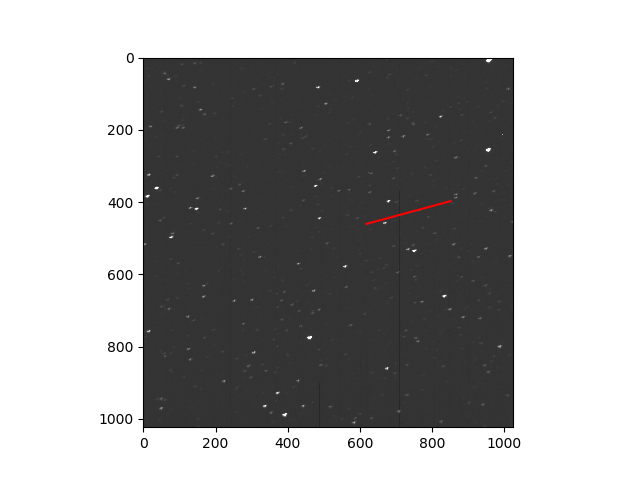
\includegraphics[width=\linewidth]{images/fig}
		  \caption{The resulting image.}
	  \label{fig:result}
	\end{figure}
	
	In the figure, we can see a recently observed (year 2017) object \emph{PR25}. The red line represents the calculated trajectory of the object. As for the objects we marked as real, see Figure \ref{fig:result}.
	
	\begin{figure}[H]
	\centering
	  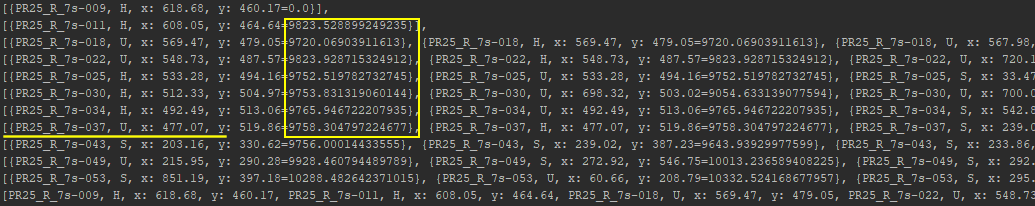
\includegraphics[width=\linewidth]{images/results_list}
		  \caption{The final objects.}
	  \label{fig:result_list}
	\end{figure}
	
	Objects above the yellow line are all confirmed as real objects. Some objects above the line are marked as unknown - in this case, this is irrelevant and is caused by incorrect input data. As is visible, the second object to the right is the next object in the \emph{bin} mentioned in Chapter \ref{chap:design}, Subsection \ref{subsec:tracklet}, and is identical to the one marked as unknown and is marked as real. More to the right, there are other objects which are considered less likely to be a real object and therefore are further in the \emph{bin}.
	
	The image perfectly shows how powerful filters and thresholds are; values in the yellow rectangle represent the baseline values compared in the algorithm and are mentioned in Chapter \ref{chap:proposed_solutions}, Section \ref{sec:linear_regression}. Also, as is visible from the last three entries, some fake objects might pass through filters and thresholds and are left for IOD, mentioned in Chapter \ref{chap:proposed_solutions}, Section \ref{sec:IDO}, to remove.
	
	The image further represents that now we have successfully created a tracklet from 8 objects out of 11 images, which is 72\% rate of success and can be improved by fine tuning threshold values. We have similar, or even higher, success rate on other tested objects not included in this document.